\documentclass[aspectratio=169]{beamer}
\usetheme{Madrid}
\usepackage{booktabs}
\usepackage{graphicx}

\title{LEBench on one virtual machine}
\subtitle{SOSP 2019, Ren et al.}
\author{Haoyu Zou \quad 5260000157}
\institute{CS340 Operating Systems}
\date{3 November 2026}

\begin{document}

\begin{frame}
\titlepage
\end{frame}

\begin{frame}{What the paper claims}
\begin{itemize}
\item Core kernel operations got slower from Linux 3.0 to 4.20 (Figure 1).
\item Big write and big munmap are the exceptions.
\item Eleven causes cover the jumps: security, features, and bad config (Table 3, Figure 2).
\item Turning them off speeds Redis, Apache, and Nginx (Section 5).
\end{itemize}
We test the first claim on the authors' kernel list, and one security switch as the extension. The applications are not run.
\end{frame}

\begin{frame}{What actually runs}
\begin{itemize}
\item Unchanged measurement code from LEBench commit \texttt{6aa7801}.
\item Same K-best rule: five samples within 5\%, timed with \texttt{clock\_gettime}.
\item Shorter loops (\texttt{BASE\_ITER} 40) so each boot can be repeated three times.
\item Ubuntu 16.04.6 in VirtualBox, legacy BIOS, disk on \texttt{D:}.
\item One \texttt{grub-reboot} per kernel. A panic falls back to 4.4.0-210.
\end{itemize}
\end{frame}

\begin{frame}{Why the numbers are not the paper's numbers}
\begin{itemize}
\item Guest: 2 vCPUs, 4\,GB, virtual disk, memory integrity on the host.
\item CPU: i7-13700H. Meltdown: not affected.
\item The paper's server is a Xeon E5-2630 v3 with 128\,GB.
\item We compare kernels to each other on this guest. We do not match the paper's nanoseconds.
\end{itemize}
\end{frame}

\begin{frame}{Extension: one switch, \texttt{nopti}}
Same kernel (4.4.0-210), same binary, command line only.
\begin{itemize}
\item getpid 314\,ns vs 295\,ns. The intervals overlap.
\item small read, send, recv, select, poll, and epoll also overlap.
\item fork 93\,$\mu$s vs 254\,$\mu$s. The intervals do not overlap, and the direction is the wrong one for a KPTI tax.
\item \texttt{/sys/.../meltdown} says ``Not affected'' on both boots.
\end{itemize}
The full table is in the report.
\end{frame}

\begin{frame}{What \texttt{nopti} shows}
\begin{itemize}
\item The vulnerability file says this CPU is not affected by Meltdown.
\item getpid, read, send, and recv move by less than the run-to-run spread.
\item fork is slower with \texttt{nopti}, which is not the paper's KPTI story.
\item The KPTI tax is not reproduced here. The CPU never pays it.
\end{itemize}
\end{frame}

\begin{frame}{Extension: batch \texttt{getpid}}
One change. Time 1{,}000 calls, divide by 1{,}000. Same K-best, same machine.
\begin{itemize}
\item 4.0.5: 245 $\pm$ 0 ns down to 129 $\pm$ 0 ns. The intervals do not overlap.
\item 4.4.0-210: 314 $\pm$ 39 ns down to 127 $\pm$ 40 ns.
\item After batching, those two kernels overlap. The single-shot slowdown does not.
\item The empty clock pair on 4.0.5 is about 130 ns. The old \texttt{getpid} row was mostly that pair.
\end{itemize}
\end{frame}

\begin{frame}{Across kernels}
Across 627 later-kernel measurements, 271 (43\%) have a higher mean than the same test on 4.0.5 and 76 (12\%) have a mean at least 50\% higher. 117 of those measurements have non-overlapping mean$\pm$stdev intervals and a higher mean, which is the bar used in the analysis.


\IfFileExists{generated/relative_latency.pdf}{%
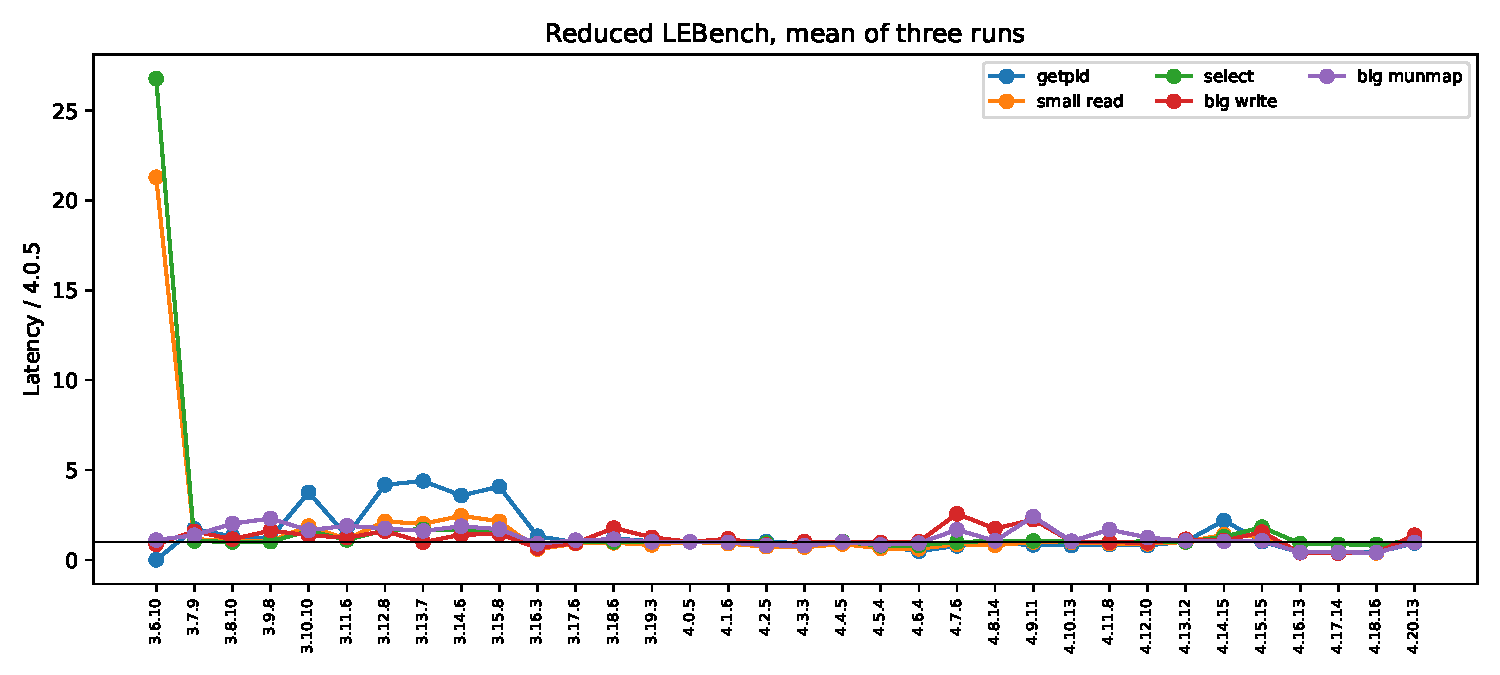
\includegraphics[width=\linewidth,height=0.55\textheight,keepaspectratio]{generated/relative_latency.pdf}
}{The relative-latency figure is written when 4.0.5 and a later kernel both have three runs.}
\end{frame}

\begin{frame}{A rewrite we did not use}
A second C suite reimplemented the tests with \texttt{rdtsc} and had an empty result table.
\begin{itemize}
\item \texttt{rdtsc} is the wrong clock on this hypervisor.
\item \texttt{select} allocates inside the timed region.
\item Context switch is one average, not K-best, and is not run at priority $-20$.
\item It had not been executed on Linux.
\end{itemize}
The course tree calls \texttt{OS\_Eval} instead of replacing it.
\end{frame}

\begin{frame}{Verdict}
34 of 41 listed kernels finished three runs. 3.0.7--3.5.4 never answered sshd. 4.19.11 had no published modules package.
\begin{itemize}
\item Claim 1: not supported here. 43\% of later-kernel means are higher than our 4.0.5; 12\% are at least 50\% higher.
\item getpid is clearly faster on 9 of 19 later kernels, and slower on 2.
\item Claim 2: \texttt{nopti} does not reproduce the KPTI tax. This CPU is not affected.
\item Claim 3: not run, so inconclusive.
\item Overall: partially reproduced. The missing piece is the paper's own conclusion, not the harness.
\end{itemize}
\end{frame}

\begin{frame}{What failed quietly}
\begin{itemize}
\item A copied benchmark still prints a number when the timer is wrong.
\item A kernel package can install and then never reach sshd.
\item Both have to be in the log: a CSV, or a boot-failure line.
\item Upstream \texttt{grub-install} onto a partition is not used. It can overwrite the wrong disk.
\end{itemize}
\end{frame}

\end{document}
